\documentclass[12pt,pra,aps]{revtex4}
\usepackage[dvipdfmx]{graphicx}
\usepackage[dvipdfmx]{color}
\usepackage{float}
\usepackage{rotating}
\usepackage{array}
\usepackage{amsmath}
\usepackage{multirow}
\usepackage{setspace}
\usepackage{braket}
\usepackage{epstopdf}
\usepackage{moreverb}
\usepackage{wrapfig}

\usepackage{color}                            
                                              
\newcommand{\red}[1]{\textcolor{red}{#1}}     
\newcommand{\blue}[1]{\textcolor{blue}{#1}}

\newcommand{\boxz}[1]{\boxed{\phantom{\text{#1}}}}
\newcommand{\boxa}[1]{\boxed{\phantom{}}}

%%\renewcommand{\baselinestretch}{2.0}

\renewcommand{\thefigure}{S\arabic{figure}}
\renewcommand{\thetable}{S\arabic{table}}

\begin{document}
\title{量子論と波動方程式}
\author{齋藤 雅明 \\ 量子化学研究室 \\ email: masa.saitow@chem.nagoya-u.ac.jp}

\maketitle

% Nakai & Ando, p. 87
\noindent
{\bf 問題1.} 次の共役二重結合をもつ1価の有機色素分子は、分子鎖の長さに対応する$k$の値 ($k=0\cdots 3$) が1増すごとに吸収する光の波長がおよそ100nmずつ長くなることが知られている。この現象は、$\pi$電子を自由電子模型により取り扱うことで理解される。このとき以下の問いに答えよ。

\noindent
{\bf 1.(a)} 長さ$L$の一次元の無限に高いポテンシャル中の電子のSchr\"odinger方程式を解き、エネルギー準位を求めよ。電子質量は$m_e$とせよ。自由電子模型の場合、$L$は共役長に対応し、$0.60+0.25k$ nmと与えられる。また$\pi$電子数は$4+2k$である。

\noindent
{\bf 1.(b)} $k=0$の色素分子に対してHOMOおよびLUMOの軌道エネルギーを求めよ。

\noindent
{\bf 1.(c)} 光吸収によるHOMO$\rightarrow$LUMO遷移を考える。$k=0$のときの吸収エネルギーおよび吸収波長を求めよ。

\noindent
{\bf 1.(d)} $k=1,2,3$についても1.(c)と同様の計算を行い、鎖長の増加に伴う吸収波長の変化を示せ。

\begin{wrapfigure}{r}[10pt]{0.3\textwidth}
  \centering
  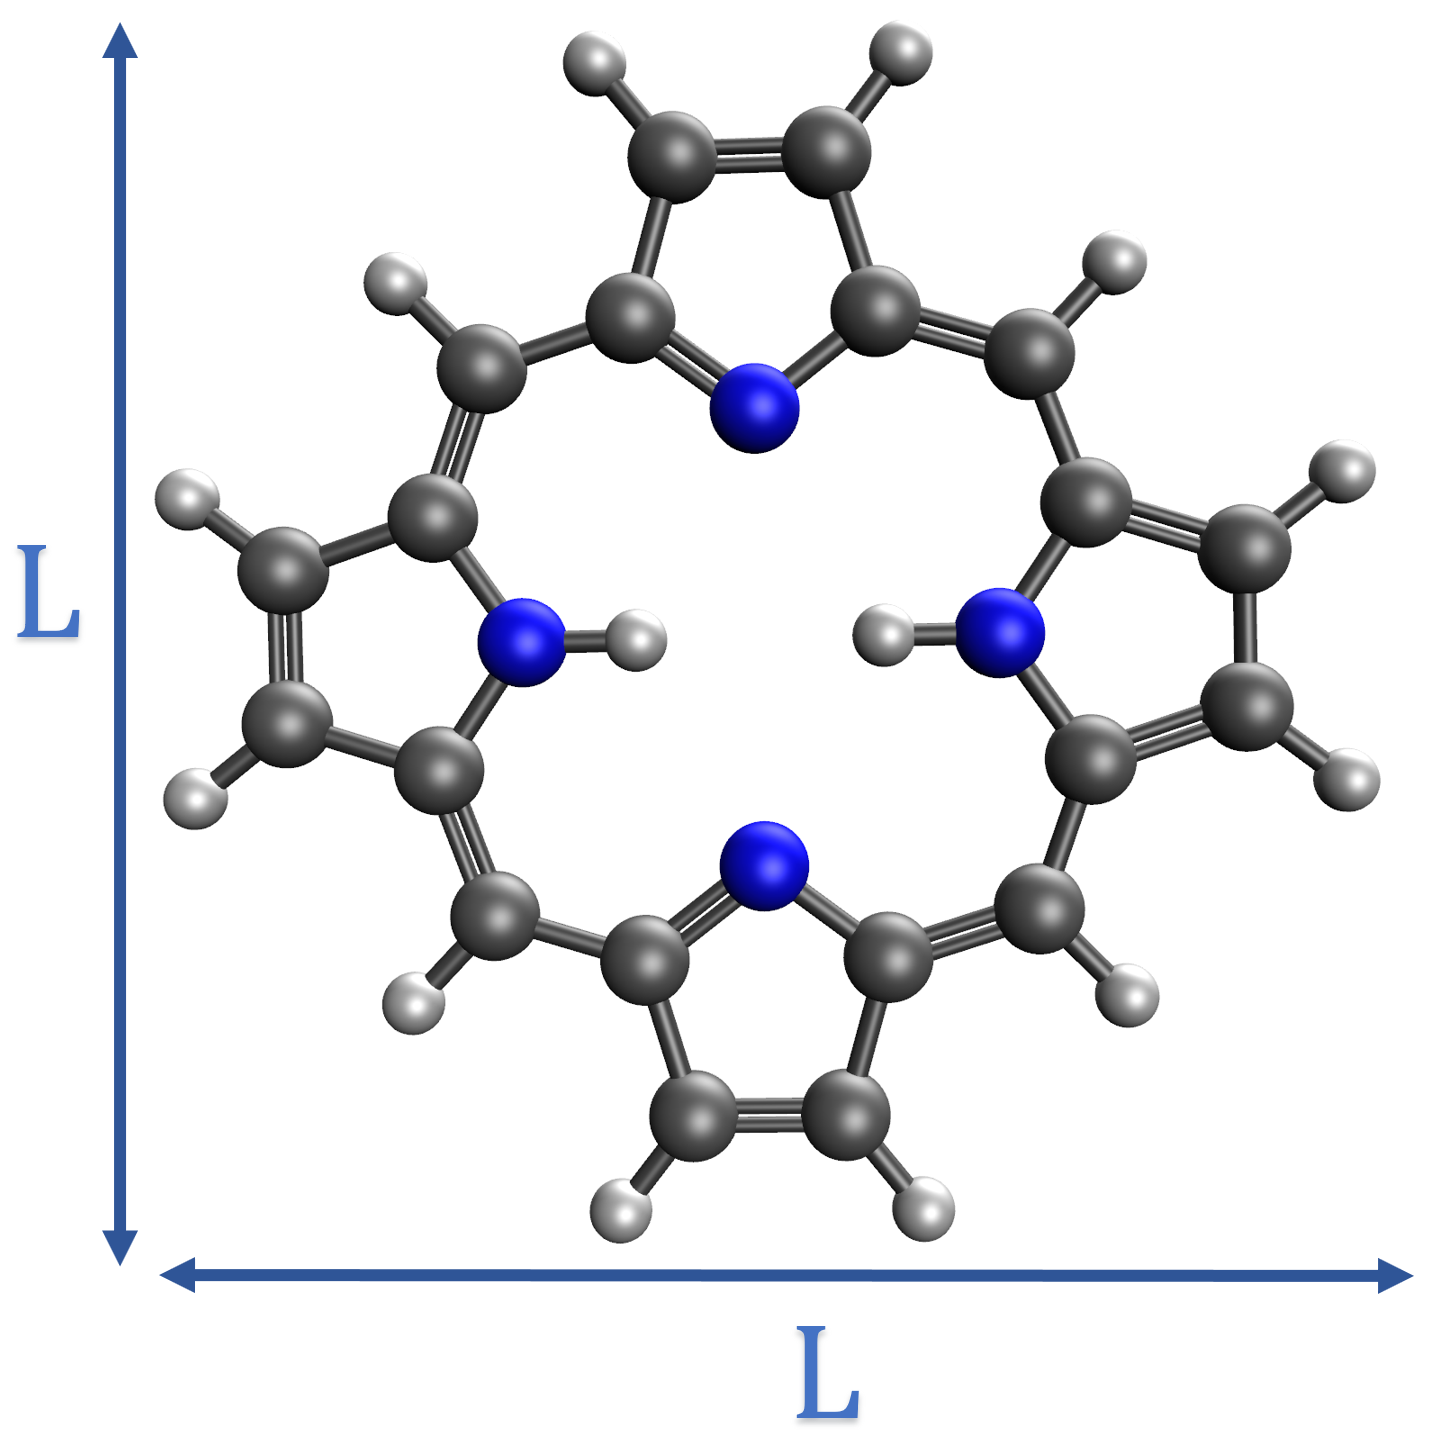
\includegraphics[width=4.5cm]{porph1.png}
  \caption{Structure of porphyrin}
\end{wrapfigure}

% Nakai & Ando, p. 88    
\noindent
{\bf 問題2.} ポルフィリン化合物は様々な波長の可視光を吸収する。これは26個の$\pi$電子が分子平面全体に広がり、$\pi$共役するためである。この現象は$\pi$電子を二次元自由電子モデルで取り扱うことで理解できる。分子平面を正方形としたときの一辺の長さを$L$($=1.00$ nm)として、以下の問いに答えよ。

\noindent
{\bf 2.(a)} エネルギー準位が
\begin{align}
  E_{n_x n_y} = \frac{(n_x^2+n_y^2)h^2}{8m_eL^2}\ \ (n_x,n_y=1,2,\cdots)
\end{align}
と与えられることを示せ。

\noindent
{\bf 2.(b)} HOMO$\rightarrow$LUMO遷移の吸収波長を求めよ。

\vspace{2cm}
\noindent
{\bf 問題3.} 力定数$k$の調和振動子ポテンシャル中の質量$m$粒子の運動を考える。また調和振動子の平衡点は$x=0$にあるものとする。このとき以下の問いに答えよ。

\noindent
{\bf 3.(a)} この粒子のハミルトニアン演算子を書き下せ。

\noindent
{\bf 3.(b)} ビリアル定理を示す(仮)

\noindent
{\bf 3.(c)} この系のエネルギーは
%    
\begin{align}
  E_\text{vib}=\hbar \omega\left(n+\frac{1}{2}\right)
\end{align}
%
と与えられる。振動量子数$n$は0以上の整数であるが、$n=0$の場合であってもエネルギーは0とはならない。このことを、3.(b)の結果を踏まえて不確定性関係の観点から考察せよ。

\noindent
{\bf 3.(d)} 作用することで座標軸を原点に対して反転させる軸反転演算子$\hat{P}$を考える。関数$f(x)$に対して
\begin{align}
  \hat{P}f(x)=f(-x)
\end{align}
として作用する。$\hat{P}$と3.(a)で求めたハミルトニアン演算子とは交換するか。即ち任意の関数$f(x)$に対して
\begin{align}
  (\hat{H}\hat{P}-\hat{P}\hat{H})f(x)=0
\end{align}
が成立することを示せ。

\noindent
{\bf 3.(e)} $v=0,1,2$に対応する調和振動波動関数に対して$\hat{P}$を作用させ、これらが$\hat{P}$の固有関数となることを示せ。またこれらの固有値を計算せよ。このことはハミルトニアン演算子を不変に保つような対象操作に対して、その固有関数が特別な対称性を示すことの一例である。

\begin{table}[h]
\caption{\label{tab:chowa}
$v=0,1,2$に対応する調和振動子波動関数。ここで$\alpha=(km)^{1/2}/\hbar$である。
}
\begin{tabular}{llll}
  \hline\hline  
  $v$          && 波動関数 \\
  \hline
  0 && $\psi_0(x)=\left(\frac{\alpha}{\pi}\right)^{1/4}e^{-\alpha x^2/2}$ \\
  1 && $\psi_1(x)=\left(\frac{4\alpha^3}{\pi}\right)^{1/4}xe^{-\alpha x^2/2}$ \\
  2 && $\psi_2(x)=\left(\frac{\alpha}{4\pi}\right)^{1/4}(2\alpha x^2-1)e^{-\alpha x^2/2}$ \\
  \hline\hline  
\end{tabular}
\end{table}


\end{document}
